% !TEX root = perelman-geometry.tex
%!TEX TS-program = pdflatex
%!TEX encoding = UTF-8 Unicode



\setchapterpreamble[o]{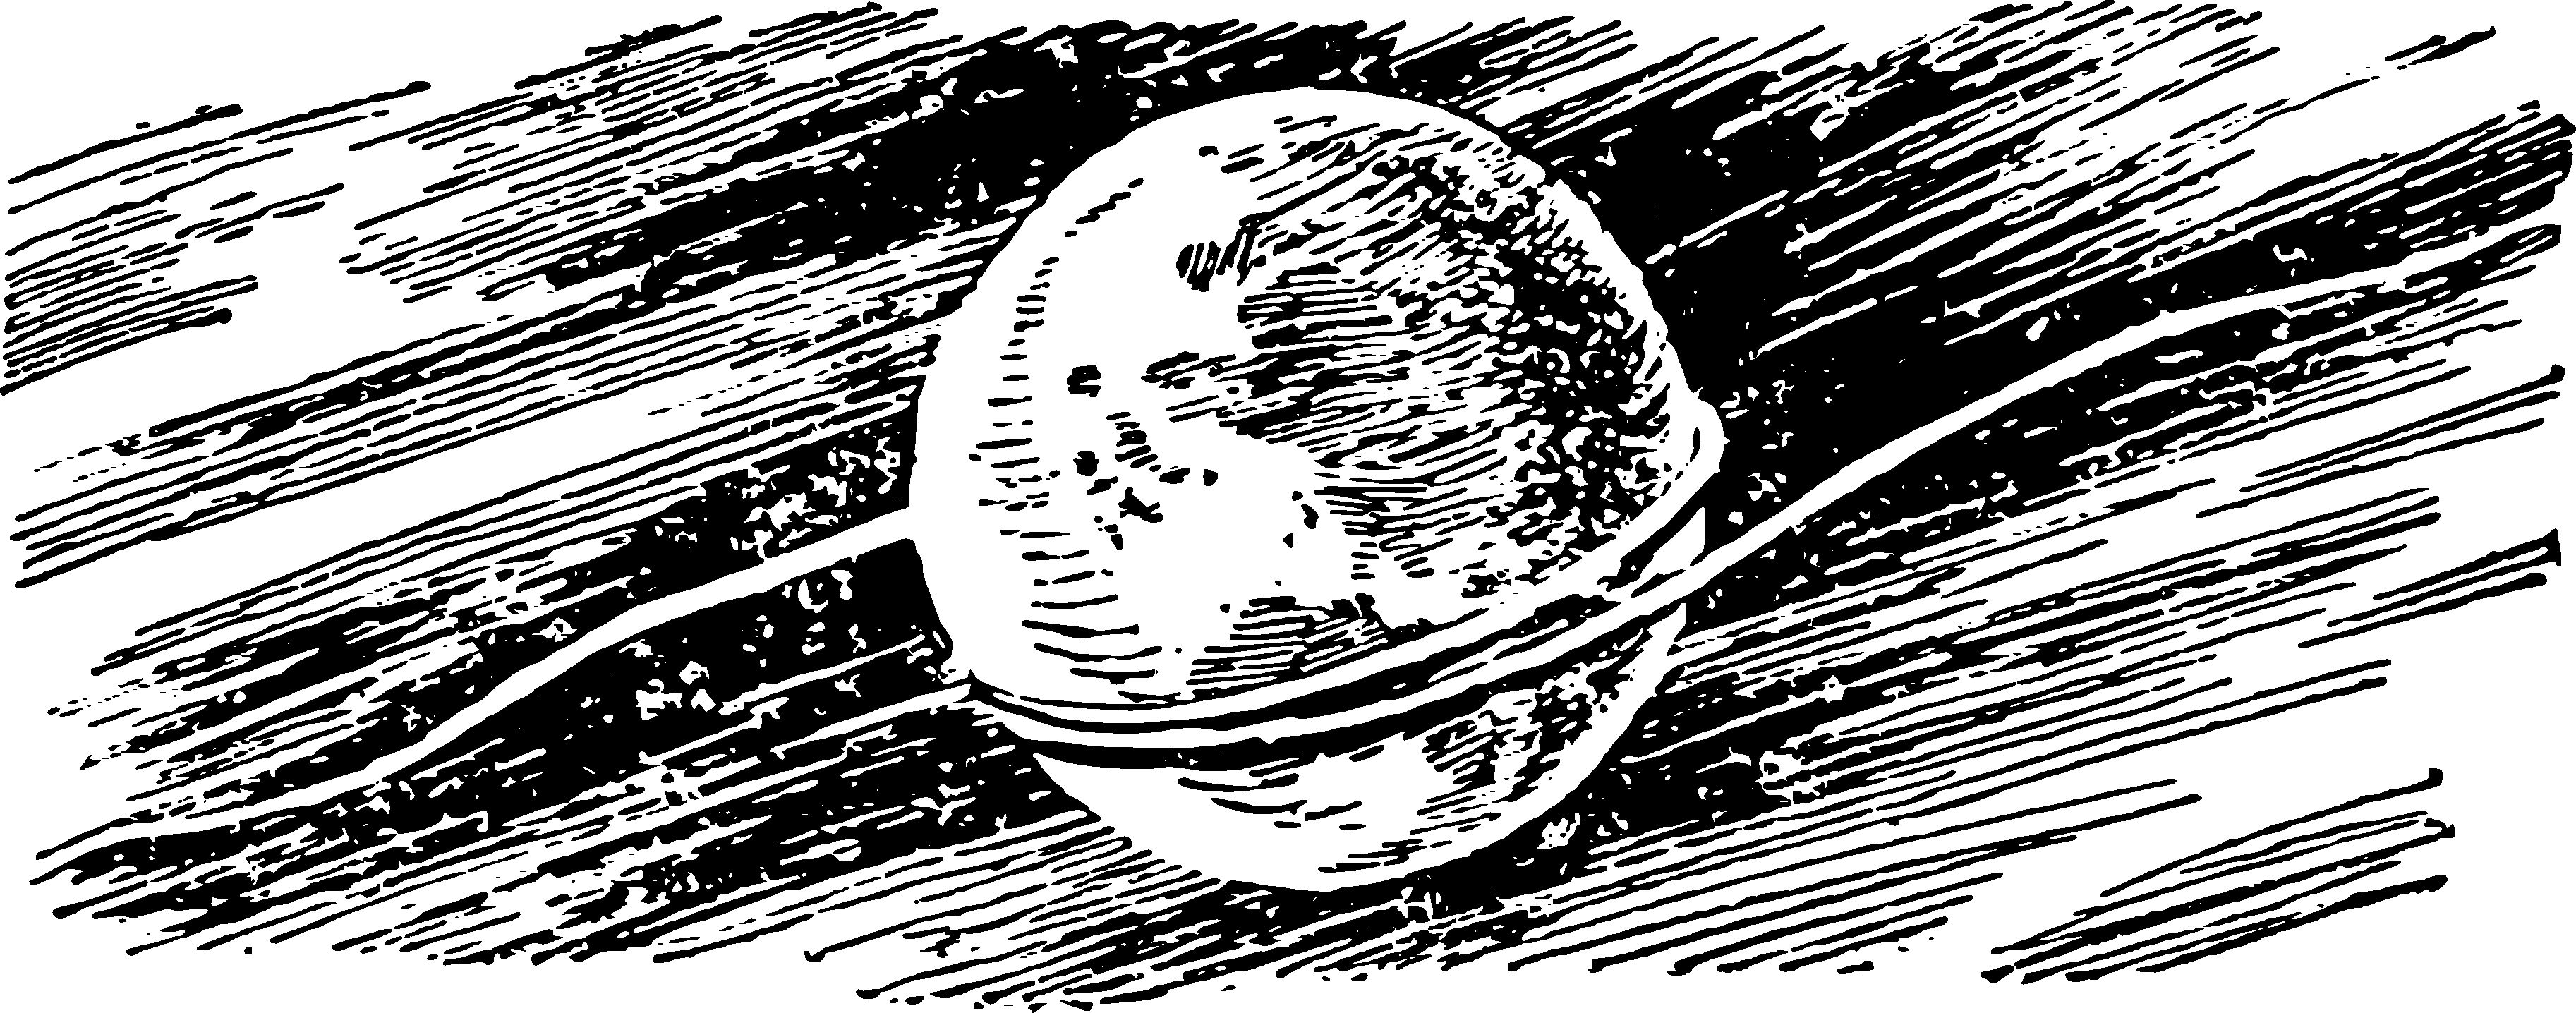
\includegraphics[width=1.2\textwidth]{figures/ch-09/fig-ch-09-head.pdf}\bigskip}

\chapter{Old And New About The Circle}
\label{ch-09}



\section{Practical geometry of the Egyptians and Romans}
\label{sec-9.1}

Any schoolchild can now calculate the circumference based on its diameter much more accurately than the wisest priest of the ancient land of pyramids or the most skilled architect of great Rome. The ancient Egyptians believed that the circumference was 3.16 times longer than the diameter, while the Romans believed it was 3.12 times longer. However, the correct ratio is 3.14159\dots{} Egyptian and Roman mathematicians established the ratio of the circumference to the diameter not through strict geometric calculation, as later mathematicians did, but simply through experience. But why did they make such errors? Couldn't they just stretch a piece of string around a circular object and then straighten the string to measure it?

Undoubtedly, they did just that, but it should not be assumed that such a method would necessarily yield good results. Imagine, for example, a vase with a round bottom with a diameter of \SI{100}{\milli\meter}. The circumference of the bottom should be \SI{314}{\milli\meter}. However, in practise, measuring with a string, you are unlikely to get this length: it is easy to make a mistake of one millimetre, and then $\pi$ will turn out to be equal to 3.13 or 3.15. And if you consider that the diameter of the vase cannot be measured perfectly accurately either, and that an error of \SI{1}{\milli\meter} is quite probable here too, then you will see that for $\pi$, quite wide limits are obtained between 
\begin{equation*}%
\frac{313}{101} \qand \frac{315}{99},
\end{equation*}
i.e., in decimal fractions, between 
\begin{equation*}%
3.09 \qand 3.18.
\end{equation*}
You see, by determining $\pi$ in this way, we can get a result that does not coincide with 3.14: once it's 3.1, another time 3.12, the third time 3.17, and so on. Among them, by chance, there may be 3.14, but in the eyes of the calculator, this number will not carry more weight than the others.

Such an empirical approach cannot provide a somewhat acceptable value for $\pi$. In this regard, it becomes more understandable why the ancient world did not know the correct ratio of the circumference to the diameter and why it took the genius of Archimedes to find the value of $3\,\frac{1}{7}$ for $\pi$ without measuring, relying solely on reasoning.



\section{``I know this and I remember it perfectly.''}
\label{sec-9.2}

In the \emph{Algebra} of the ancient Arab mathematician Mohammed ibn-Musa, we read the following lines about calculating the circumference:
\begin{quote}
The best way is to multiply the diameter by $3\,\frac{1}{7}$. This is the fastest and easiest way. God knows the best. 
\end{quote}
Now we also know that Archimedes' number $3\,\frac{1}{7}$ does not perfectly express the ratio of the circumference to the diameter. It has been theoretically proven that this ratio cannot be expressed as any exact fraction. We can only write it with some approximation, which, however, far exceeds the accuracy required for the strictest demands of practical life. The mathematician Ludolph in the 16th century, in Leiden, had the patience to calculate $\pi$ with 35 decimal places and bequeathed to have this value for $\pi$ carved on his tombstone\sidenote{At that time, the notation $\pi$ was not yet in use: it was introduced only from the middle of the 18th century by the famous Russian academician and mathematician Leonard Pavlovich Euler.}! (see \figr{fig-123}).

\begin{figure}[h!]
\centering
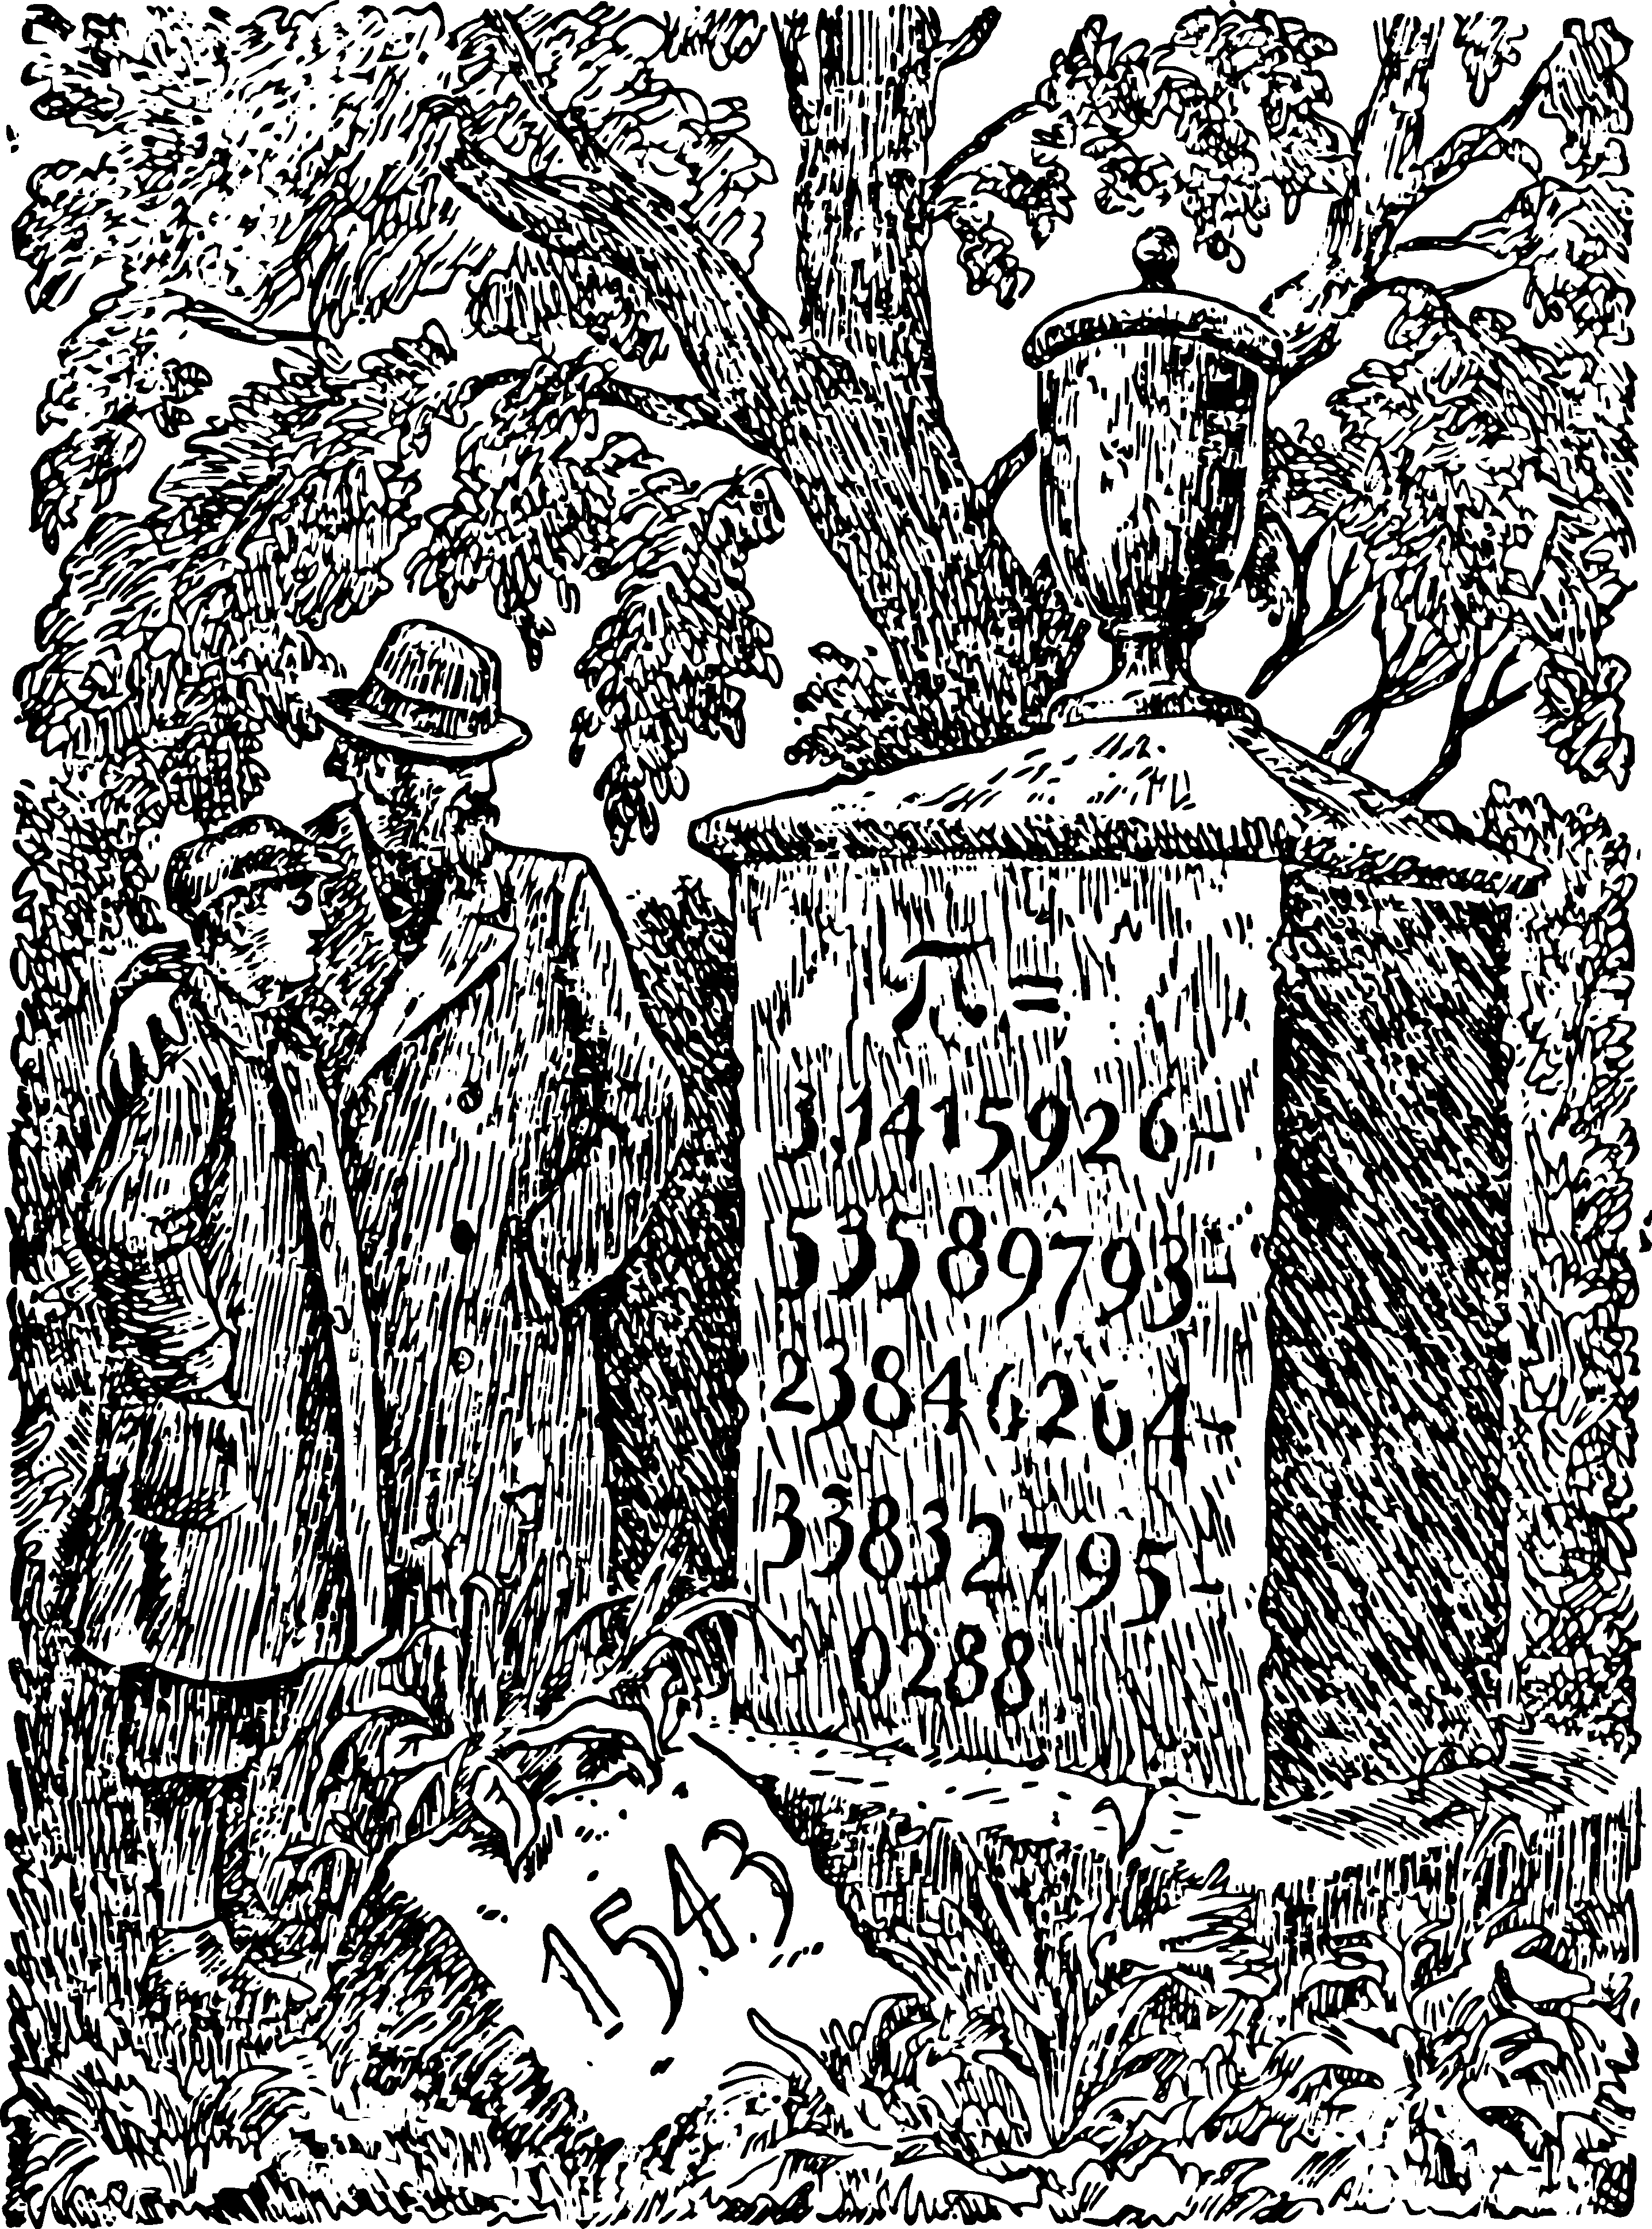
\includegraphics[width=0.7\textwidth]{figures/ch-09/fig-123.pdf}
\sidecaption{Mathematical epitaph.\label{fig-123}}
\end{figure}


Here it is: 
\begin{equation*}%
\num{3.14159265358979323846264338327950288}\dots{}
\end{equation*}
A certain Shanks in 1873 published a value of $\pi$ in which there were 707 decimal places after the comma! Such long numbers approximately expressing the value of $\pi$ have neither practical nor theoretical value. Only out of idleness and in pursuit of inflated ``records'' could there arise in our time a desire to "outdo" Shanks: in 1946-1947, Ferguson (Manchester City) and, independently of him, Weaver (from Washington) calculated 808 decimal places for the number $\pi$ and were pleased to find errors in Shanks's calculations starting from the 528th digit.\sidenote[][-2cm]{As of 2024, the value of $\pi$ has been calculated to 62,831,853,071,796 digits, that is \textbf{62 trillion} digits! For several different and modern methods to find value of $\pi$, please see the Wikipedia page \url{https://en.wikipedia.org/wiki/Pi}. -- \textsc{dm}}

If, for example, we wished to calculate the length of the Earth's equator with an accuracy of \SI{1}{\centi\meter}, assuming that we know the length of its diameter precisely, it would be sufficient for us to take only 9 digits after the decimal point in the number $\pi$. And by taking twice as many digits (18), we could calculate the circumference with a precision of not more than \SI{0.0001}{\milli\meter} (100 times smaller than the thickness of a hair!) for a circle with a radius equal to the distance from the Earth to the Sun.

Our compatriot, the mathematician Grave, vividly demonstrated the absolute uselessness of even the first hundred decimal places of $\pi$. He calculated that if we imagine a sphere with a radius equal to the distance from the Earth to Sirius, i.e., a number of kilometres equal to 132 followed by ten zeros: \num{132d10}, and fill this sphere with microbes, placing one billion (\num{d10}) microbes in each cubic millimetre of the sphere, and then arrange all these microbes in a straight line so that the distance between each pair of adjacent microbes again equals the distance from Sirius to Earth, then, taking this fantastic segment as the diameter of a circle, it would be possible to calculate the length of the resulting gigantic circumference with microscopic precision — up to \SI{0.000001}{\milli\metre}, by using 100 digits after the decimal point in the number $\pi$. French astronomer Arago correctly observes in this regard that ``in terms of accuracy, we would gain nothing if there were a relationship between the circumference and the diameter expressed by a number with complete accuracy.''

For ordinary calculations involving $\pi$, it is sufficient to remember two digits after the decimal point (3.14), and for more precise calculations, four digits (3.1416: we take the last digit as 6 instead of 5 because the following digit is greater than 5).

Small poems or vivid phrases are better retained in memory than numbers, so special poems or individual phrases are invented to memorise some numerical value of $\pi$. In works of this kind of mathematical poetry, words are chosen so that the number of letters in each word sequentially coincides with the corresponding digit of the number $\pi$.

There is a famous poem in English -- in 13 words, hence providing 12 digits after the decimal point in the number $\pi$; in German -- in 24 words, and in French, in 30 words! (and there are even ones in 126 words).

They are curious but too large, cumbersome. Among the students, E. Y. Terskov, a mathematics teacher at one of the secondary schools in the Moscow region, enjoys popularity for inventing the following stanza:

%\begin{quote}
\gl{«Это я знаю и помню прекрасно».}
{3 1 4 1 5 9} \\
(`I know this and remember it perfectly.')\sidenote[][-2cm]{This sentence and the next ones are not really translatable with the number of characters in the words intact and corresponding to the numbers in $\pi$. I am giving the translations in English which do not match. I am also giving some alternative mnemonics in English. -- \textsc{dm}}
%\end{quote}

% See the discussion at https://tex.stackexchange.com/questions/717912/how-to-align-numbers-to-words-of-a-sentence-in-the-next-line/

And one of his students, Elya Cherikover, with the resourcefulness typical of our schoolchildren, composed a witty, slightly ironic continuation:

%\begin{quote}
\gl{«Пи многие знаки мне лишни, напрасны»,}{2 6 5 3 5 8}\\
('Pi, many digits are unnecessary for me, in vain,') 
%\end{quote}
In total, a twelve-word couplet is obtained:

\gl{«Это я знаю и помню прекрасно, Пи многие знаки мне лишни, напрасны».}{3 1 4 1 5 9 2 6 5 3 5 8}

(`I know this and remember it perfectly, Pi, many digits are unnecessary for me, in vain.')

The author of this book, not daring to invent a poem, in turn suggests a simple and also quite sufficient prose phrase:

«Что я знаю о кругах?» ('What do I know about circles?') -- a question, secretly containing the answer; 3.1416.

Some English mnemonics:

\gl{See I have a rhyme assisting, My feeble brain, its tasks ofttimes resisting.}{3 1 4 1 5 9 2 6 5 3 5 8 9}

\gl{Wow! I made a great discovery!}{3 1 4 1 5 9}

\gl{Can I have a small container of coffee?}{3 1 4 1 5 9 2 6}

\gl{How I want a drink, alcoholic of course, after the heavy lectures involving quantum mechanics.}{3 1 4 1 5 9 2 6 5 3 5 8 9 7 9}

A German menmonic (24 digits):

\gl{Wie o dies $\pi$, Macht ernstlich, so vielen viele Müh’! Lernt immerhin, Jünglinge, leichte Verselein, Wie so zum Beispiel dies dürfte zu merken sein.}{3 1 4 1 5 9 2 6 5 3 5 8 9 7 9 3 2 3 7 4 6 2 6 4}

A French mnemonic (30 digits):

\gl{Que j’aime à faire apprendre un nombre utile aux sages! Jmmortel Archimède, sublime ingénieur, Qui de ton jugement peut sonder la valeur? Pour moi ton problème eut de pareils avantages.}{3 1 4 1 5 9 2 6 5 3 5 8 9 7 9 3 2 3 7 4 6 2 6 4 3 3 8 3 2 7 9}

\section{Jack London's Error}
\label{sec-9.3}

The next passage from Jack London's novel \emph{The Little Lady of the Big House} provides material for geometric calculation:
\begin{quote}
In the middle of the field stood a steel pole, driven deep into the ground. From the top of the pole to the edge of the field stretched a cable, attached to a tractor. The mechanics pressed a lever -- and the engine started.

The machine moved forward on its own, describing a circle around the pole, which served as its center.

``To truly perfect the machine,'' Graham said, ``you need to turn the circle it describes into a square.''

``Yes, on a square field, this system wastes a lot of land.''

Graham made some calculations, then remarked:

``We lose approximately three acres out of every ten.''

``No less.''
\end{quote}

Readers are invited to verify this calculation.

\ans The calculation is incorrect: less than 0.3 of the total land is lost. Let's assume that the side of the square is $a$. The area of such a square is $a^{2}$. The diameter of the inscribed circle is also $a$, and its area is $\pi a^{2}/4$. The lost part of the square plot is
\begin{equation*}%
a^{2} - \frac{\pi a^2}{4} = \left(1 - \frac{\pi}{4} \right) a^{2}= 0.22 \, a^{2}.
\end{equation*}
We can see that the unused part of the square field amounts not to 30\% as the characters in the American novelist's story believed, but only about 22\%.


\section{Dropping a Needle}
\label{sec-9.4}


The most original and unexpected method for approximating the number $\pi$ is as follows. Take a short (about two centimeters) sewing needle -- preferably with a blunted tip to ensure uniform thickness -- and draw a series of thin parallel lines on a sheet of paper, with each line spaced apart by twice the length of the needle.

\begin{figure}[h!]
\centering
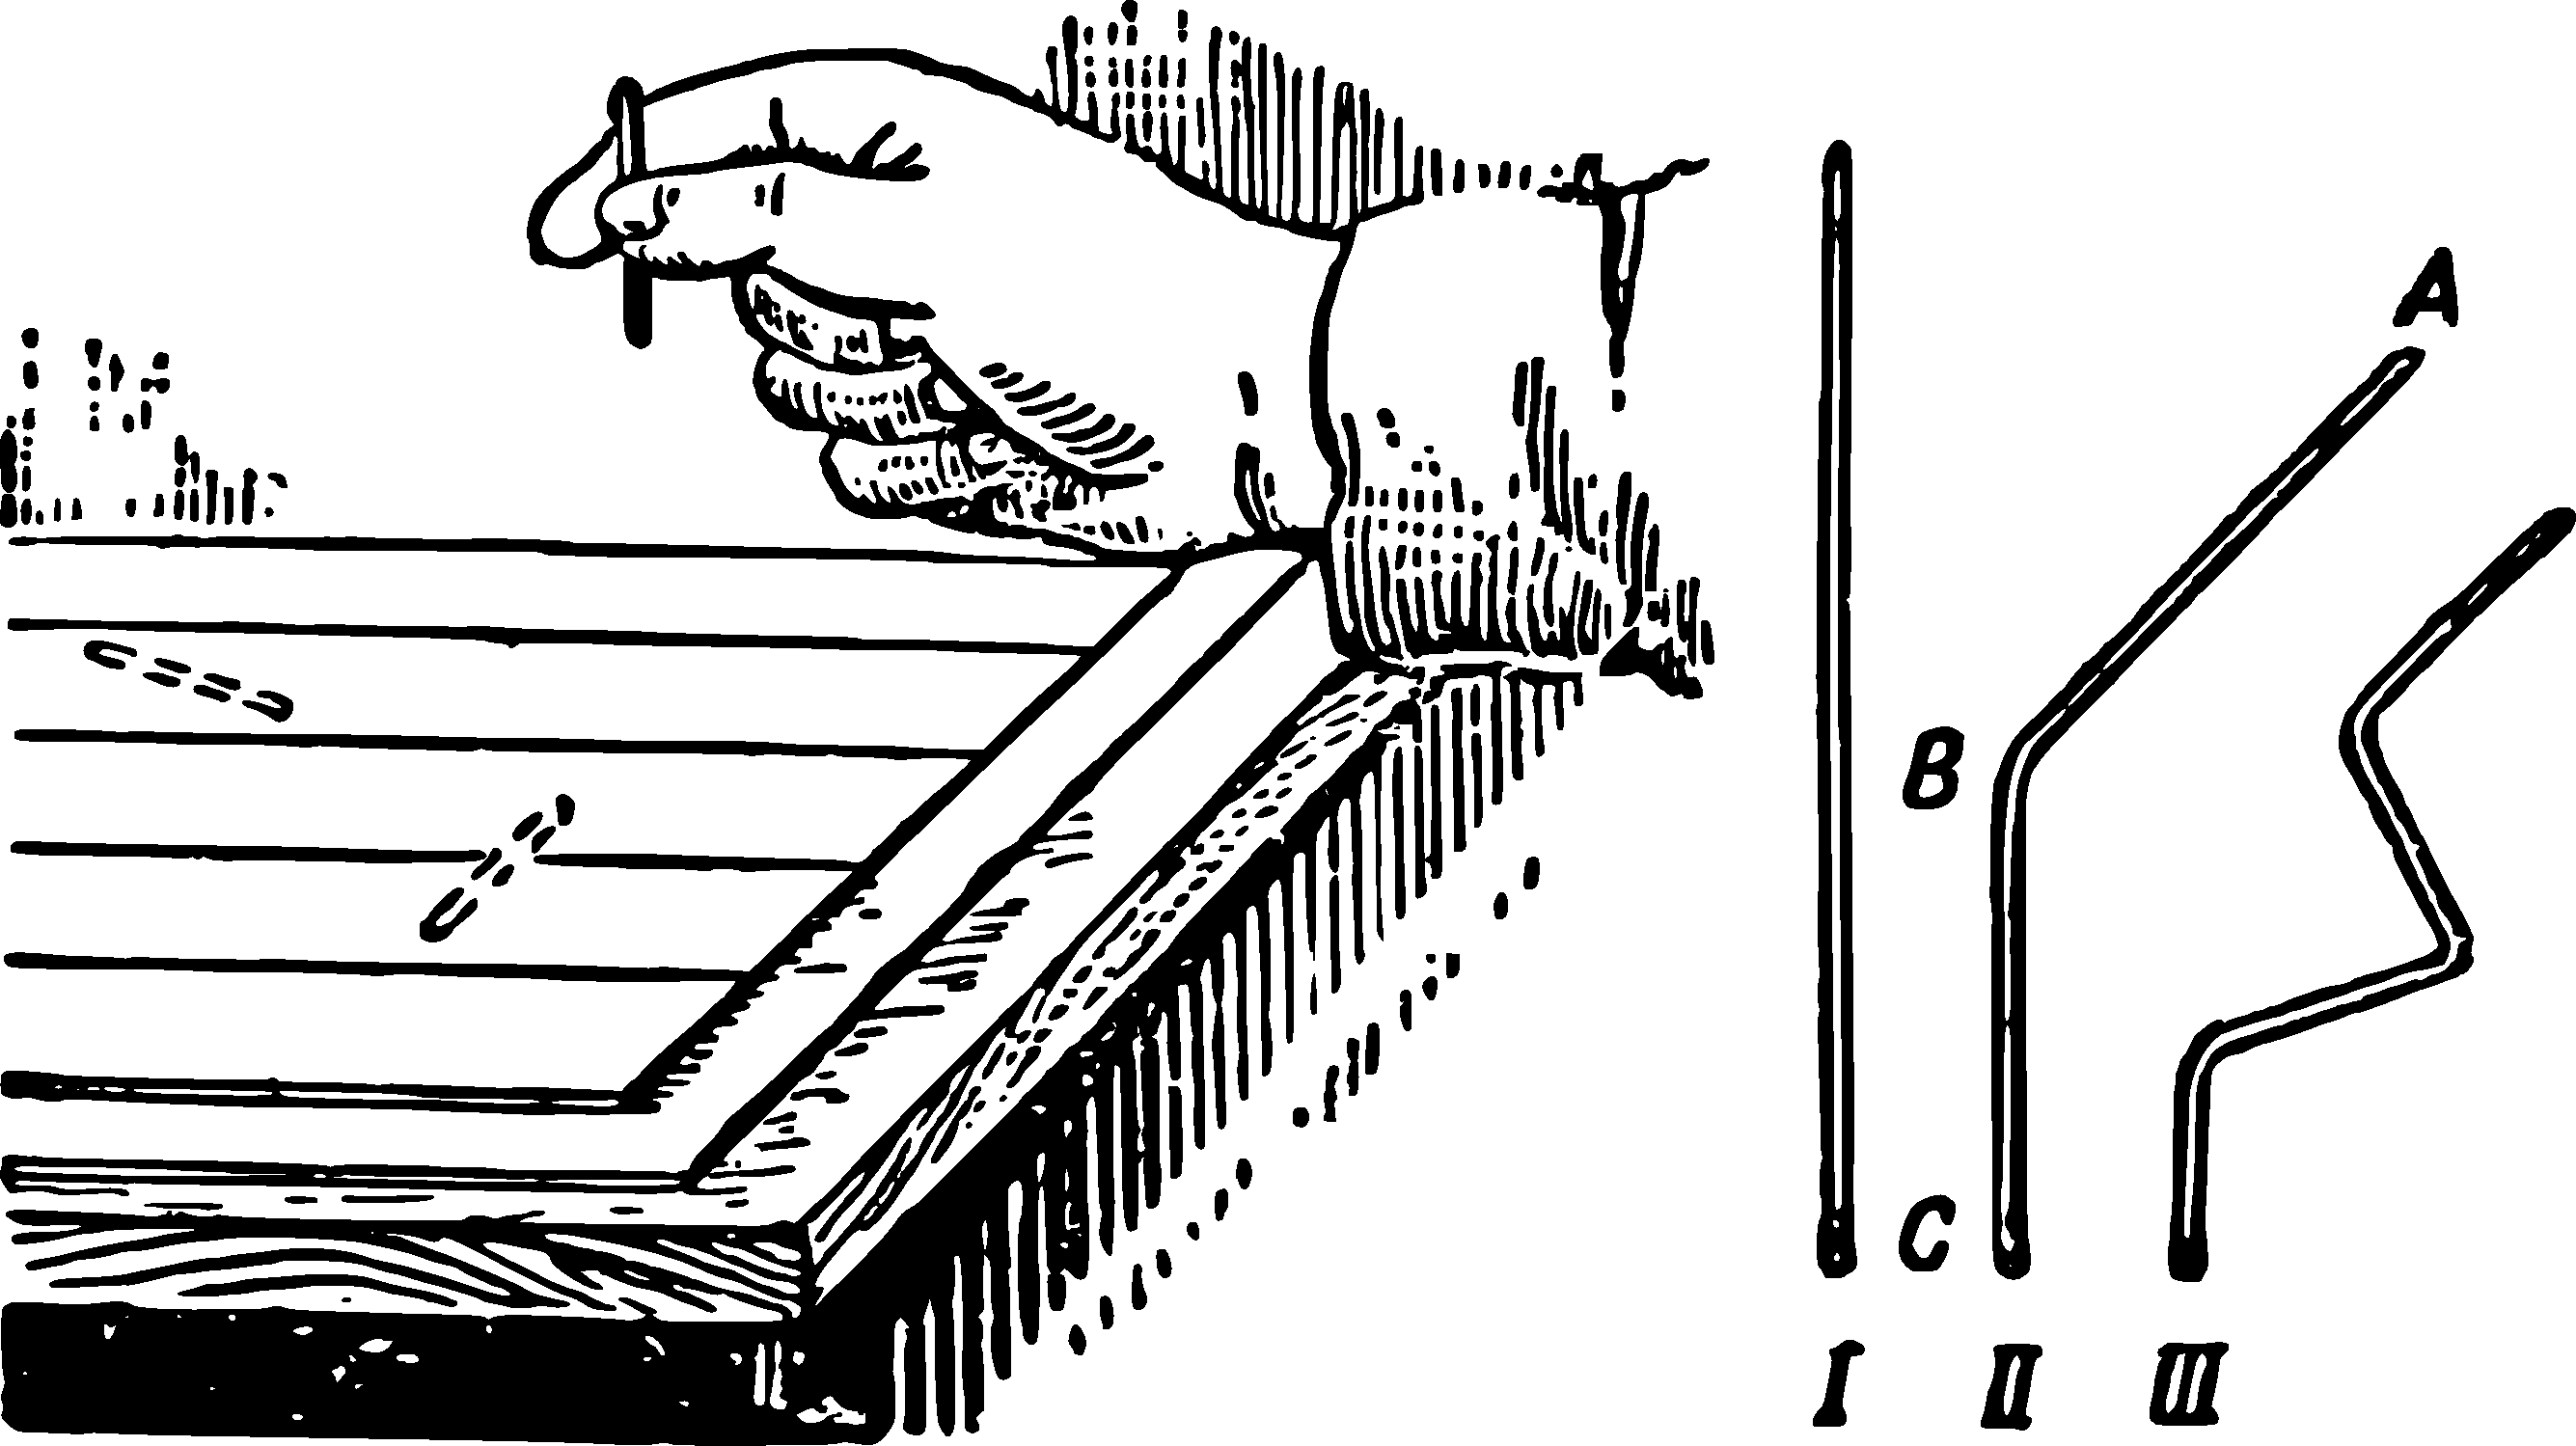
\includegraphics[width=0.9\textwidth]{figures/ch-09/fig-124.pdf}
\sidecaption{Buffon's needle-throwing experiment.\label{fig-124}}
\end{figure}

Then, drop the needle onto the paper from a certain (arbitrary) height and observe whether the needle crosses one of the lines or not (see \figr{fig-124}, left). To prevent the needle from bouncing, place a piece of thin paper or cloth under the paper sheet. Repeat the dropping of the needle many times, for example a hundred or, even better, a thousand times, each time noting whether there was a crossing or not.\sidenote{The intersection should also be considered the case when the needle only rests against the end of the drawn line.} If you then divide the total number of needle drops by the number of instances where a crossing was observed, the result should approximate the value of $\pi$, more or less accurately.

Let's explain why this happens. Let the most likely number of needle crossings be denoted as  $K$, and the length of our needle be \SI{20}{\milli\meter}. In the case of a crossing, the point of intersection must, of course, lie on one of these millimeters, and no one millimeter, nor any part of the needle, has any advantage in this regard over the others. Therefore, the most likely number of crossings for each individual millimeter is $K/20$. For a segment of the needle of \SI{3}{\milli\meter}, it is $ 3K/20$, for a segment of \SI{11}{\milli\meter} -- $ 11K/20$, and so on. In other words, the most likely number of crossings is directly proportional to the length of the needle.

This proportionality is maintained even if the needle is bent. Let the needle be bent in the form shown in figure \figr{fig-124}, (\emph{II} right), with segment $AB = \SI{11}{\milli\meter}$ and $BC = \SI{9}{\milli\meter}$. For segment $AB$, the most likely number of crossings is $11K/20$, and for segment $BC$ it is $9K/20$. For the entire needle it is $ 11K/20 + 9K/20$, which still equals $K$. We can bend the needle in a more intricate way (\figr{fig-124}, (\emph{III} right)) -- this would not change the number of crossings. (Note that with a bent needle, crossings are possible with two or more parts of the needle at once; such crossings should be counted as 2, 8, etc., because the first is counted for one part of the needle, the second for another, and so on.)

Now imagine that we are dropping a needle, bent into the shape of a circle with a diameter equal to the distance between the lines (it is twice the length of our needle). Such a ring must intersect any line twice each time (or touch two lines once each -- in any case, two encounters occur). If the total number of drops is $N$, then the number of encounters is $2N$. Our straight needle is shorter than this ring by as many times as the radius is less than the circumference, which is $2\pi$ times. But we have already established that the most likely number of crossings is proportional to the length of the needle. Therefore, the most likely number $(K)$ of crossings of our needle should be less than $2M$ by $2\pi$ times, i.e., equal to $N/\pi$. Hence,
\begin{equation*}%
 \pi = \frac{\text{number of drops}}{\text{number of crossings}}.\end{equation*}

The more drops observed, the more accurate the expression for $\pi$ becomes. The Swiss astronomer R. Wolff in the middle of the last century observed 5000 needle drops on grid paper and obtained $\pi$ as 3.159\dots{} an expression, however, less precise than the Archimedean number.

As you can see, the ratio of the circumference to the diameter is determined here experimentally, and what is more curious -- neither a circle nor a diameter is drawn, meaning no compass is used. A person with no knowledge of geometry or even circles can determine $\pi$ using this method if they patiently perform a very large number of needle drops.

%\vspace{2cm}

\section{Straightening a Circle Problem}
\label{sec-9.5}

\begin{marginfigure}
\centering
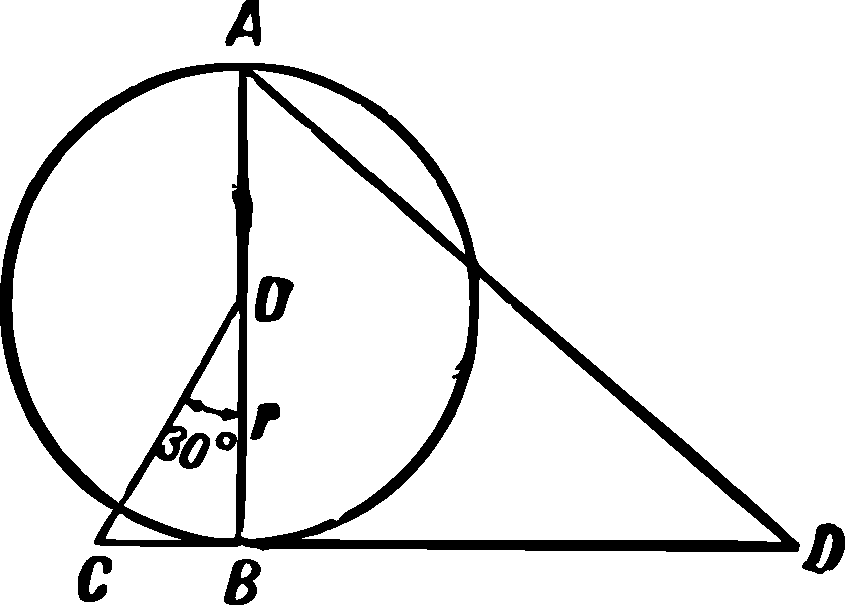
\includegraphics[width=\textwidth]{figures/ch-09/fig-125.pdf}
\sidecaption{An approximate geometric method of rectifying a circle.\label{fig-125}}
\end{marginfigure}

For many practical purposes, it is sufficient to take $\pi$ as 3 and  1/7 straighten the circle by laying out its diameter on any straight line 3 \, 1/7 times (dividing the segment into seven equal parts can be done quite accurately, as is well known). There are other approximate methods for straightening a circle used in practise by craftsmen such as carpenters, tinsmiths, and so on. We won't discuss them here, but we'll mention one fairly simple method of straightening that yields results with extremely high accuracy.



If it is necessary to straighten a circle $O$ with radius $r$ (see \figr{fig-125}), then draw the diameter $AB$, and at point $B$, draw line $CD$ perpendicular to it. From the centre $O$, draw line $OC$ at an \ang{30} angle to $AB$. Then, on line $CD$ from point $C$, mark off three radii of the given circle and connect the resulting point $D$ to $A$: the length of segment $AD$ equals the length of half the circumference. If segment $AD$ is doubled in length, an approximately straightened circle $O$ is obtained. The error is less than $0.0002\, r$.

On what basis is this construction founded?

\ans According to the Pythagorean theorem, 
\begin{equation*}%
CB^{2} + OB^{2} = OC^{2}.
\end{equation*}
Denoting the radius $OB$ as $r$ and considering that $CB = OC/2$ (as a leg, lying opposite an \ang{30} angle), we get: 
\begin{align*}%
CB^{2} + r^{2}  & = 4CB^{2}, \,\, \text{from which}\\
CB & = \frac{r \sqrt{3}}{3}.
\end{align*}
Next, in triangle $ABD$:
\begin{align*}%
BD & =  CD - CB = 3r - \frac{r\sqrt{3}}{3}.\\
AD & = \sqrt{BD^{2} + 4r^{2}} = \sqrt{\left( 3r - \frac{r \sqrt{3}}{3} \right)^{2} + 4r^{2}} \\
& = \sqrt{9r^{3} - 2r^{2}\sqrt{3} + r^{2}/3 + 4r^{2}} \\
& = 3.14153\, r.
\end{align*}
Comparing this result with one obtained with high precision for $\pi$ (approximately $( \pi = 3.14153)$, we see that the difference is only $0.00006\, r$. If we were to straighten a circle with a radius of 1 unit using this method, the error would be only 0.00006 meters for the semicircle, and for the full circle, it would be 0.00012 meters, or 0.12 millimetres (roughly three times the thickness of a hair).


\section{Squaring the Circle}
\label{sec-9.6}

It is unlikely that any reader has never heard of the ``squaring of the circle'' -- that most famous problem in geometry that mathematicians have been working on for twenty centuries. I am even confident that among the readers there are those who have tried to solve this problem themselves. However, even more readers may wonder what exactly the difficulty lies in resolving this classic unsolvable problem. Many, accustomed to repeating from others that the problem of squaring the circle is unsolvable, do not have a clear understanding of the essence of the problem or the difficulty of its resolution.

In mathematics, there are many problems much more interesting both theoretically and practically than the problem of squaring the circle. However, none has gained such popularity as this problem, which has long become a byword. For two millennia, outstanding professional mathematicians and countless crowds of amateurs have worked on it.

To square the circle" means to draw a square whose area is exactly equal to the area of a given circle. Practically, this problem arises very often, but precisely in practise, it can be solved with any degree of accuracy. The famous ancient problem, however, requires that the drawing be done perfectly using only two types of drawing operations: 
\begin{enumerate}
\item drawing a circle of a given radius around a given point; 
\item drawing a straight line through two given points.
\end{enumerate}
In short, it is necessary to make a drawing using only two drawing instruments: a compass and a straightedge.


In other words, it is necessary to make a drawing using only two drawing instruments: a compass and a straightedge.

Among non-mathematicians, there is a widespread belief that all the difficulty lies in the fact that the ratio of the circumference to its diameter (the famous number π) cannot be expressed by a finite number of digits. This is true only to the extent that the solvability of the problem depends on the peculiar nature of the number $\pi$. Indeed: transforming a rectangle into a square with equal area is an easily and precisely solvable problem. But the problem of squaring the circle is reduced to constructing -- with a compass and a straightedge -- a rectangle equal in area to the given circle. From the formula for the area of a circle, $S = \pi r^2$, or (which is the same thing) $S = \pi \times r \times r$, it is clear that the area of the circle is equal to the area of such a rectangle, where one side is $r$ and the other is $\pi$ times larger. As you know, $\pi$ is not exactly equal to 3 \, 1/7, or 3.14, or even 3.14159. The series of digits expressing this number goes to infinity.

The particularity of the number $\pi$, its irrationality\sidenote{The peculiarity of an irrational number is that it cannot be expressed as any exact fraction.}, was established by mathematicians Lambert and Legendre back in the 18th century. Yet, the knowledge of the irrationality of $\pi$ did not stop the efforts of those versed in mathematics, the ``quadraturists''. They understood that the irrationality of $\pi$ itself does not make the problem hopeless. There are irrational numbers that geometry can ``construct'' perfectly accurately. For example, suppose we need to draw a segment that is longer than a given one by $\sqrt{2}$ times. The number $\sqrt{2}$, like $\pi$, is irrational. Nevertheless, nothing could be easier than drawing the desired segment: let's remember that $\sqrt{2}$ is the side of a square inscribed in a circle with a radius of 1, because it amounts to constructing a regular 64-gon.



Every schoolchild also easily copes with constructing the segment $ a \sqrt{3}$ (the side of an equilateral inscribed triangle). Even constructing such a seemingly complex irrational expression presents no particular difficulty:
\begin{equation*}%
\sqrt{2 - \sqrt{2 + \sqrt{2 + \sqrt{2 +\sqrt{2}}}}}
\end{equation*}
As we can see, an irrational multiplier, entering into the expression, does not always render this expression impossible to construct with a compass and straightedge. The unsolvability of squaring the circle is not entirely due to the fact that the number $\pi$ is irrational, but to another peculiarity of this same number. Namely, the number $\pi$ is not algebraic, i.e., it cannot be obtained as the solution to any equation with rational coefficients. Such numbers are called ``transcendental''.

A mathematician of the 19th century proved that the number $\pi$ is transcendental. This expression for $\pi$ would solve the problem of squaring the circle if the number of operations involved were finite (then the expression could be geometrically constructed). But since the number of square root extractions in this expression is infinite, Vieta's expression does not help the cause.

So, the unsolvability of the problem of squaring the circle is due to the transcendence of the number $\pi$, i.e., it cannot be the result of solving an equation with rational coefficients. This peculiarity of the number $\pi$ was rigorously prooven in 1889 by the German mathematician Lindemann. In essence, this scientist should be considered the only person who solved the squaring of the circle problem, despite the fact that his solution is negative -- it asserts that the desired construction is geometrically impossible. Thus, in 1889 the centuries-long efforts of mathematicians in this direction were concluded; however, unfortunately, the fruitless attempts of numerous amateurs, insufficiently familiar with the problem, have not ceased.

This is the state of affairs in theory. As for practise, it does not require an exact resolution of this famous problem at all. The belief of many that solving the problem of squaring the circle would have a huge significance for practical life is a profound misconception. For everyday needs, it is perfectly sufficient to have good approximate solutions to this problem.


Practically, the quest for squaring the circle became futile once the first 7-8 accurate digits of the number $\pi$ were found. For the needs of practical life, it is entirely sufficient to know that $\pi$ is approximately equal to 3.1415926. No measurement of length can provide a result expressed in more than seven significant digits. Therefore, having more than eight digits for $\pi$ is useless: it does not improve the precision of calculations\sidenote{See \emph{Entertaining Mathematics} by Yakov I. Perelman.}. Even if the radius is expressed with seven significant digits, the circumference will not contain more than seven reliable digits, even if $\pi$ is taken to a hundred digits. The fact that ancient mathematicians expended enormous effort to obtain possibly longer values of $\pi$ has no practical significance. Moreover, the scientific value of these works is negligible. It's simply a matter of patience. If you have the inclination and leisure, you can find up to 1000 digits for $\pi$ using, for example, the following infinite series discovered by Leibniz\sidenote{A lot of patience would be required for such a calculation because to obtain, for example, a six-digit $\pi$ , it would be necessary to take in the specified series not a few, not a little -- 2,000,000 terms.}:
\begin{equation*}%
\frac{\pi}{4} = 1 - \frac{1}{3} + \frac{1}{5} - \frac{1}{7} + \frac{1}{9} - \frac{1}{11} + \ldots{}
\end{equation*}
But this would be an unnecessary arithmetic exercise, far from contributing to the resolution of the famous geometric problem.

The French astronomer Arago, mentioned earlier, wrote the following about this:
\begin{quote}
The seekers of the squaring of the circle continue to engage in solving a problem whose impossibility is now positively proven and which, even if it could be achieved, would be of no practical interest. It is not worth dwelling on this subject: the mentally ill, striving for the discovery of the squaring of the circle, are not swayed by any arguments. This mental illness has existed since ancient times.
\end{quote}
And he ironically concludes:
\begin{quote}
The academies of all countries, fighting against the seekers of quadrature, have noticed that this disease usually intensifies in the spring.
\end{quote}

\begin{center}
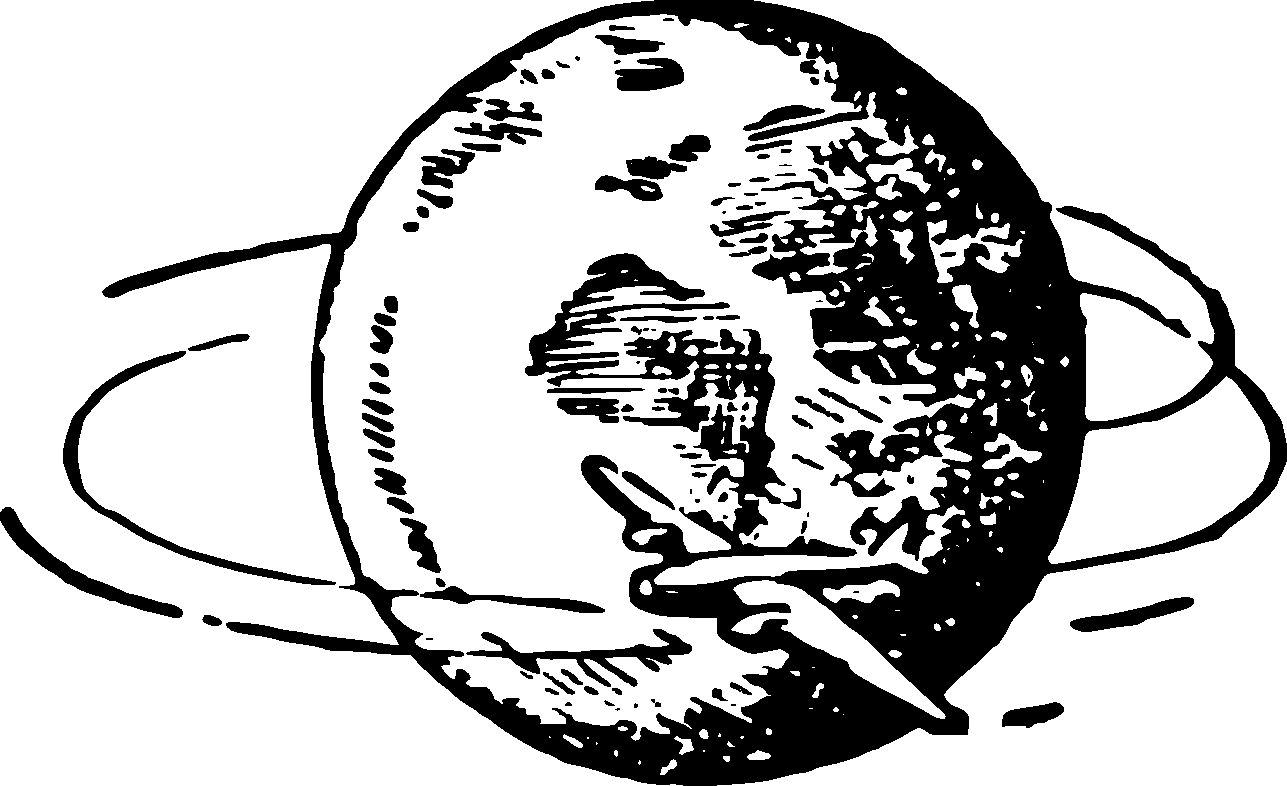
\includegraphics[width=0.3\textwidth]{figures/ch-09/fig-ch-09-tail.pdf}
\end{center}


















